\section{Introduction}

An important step of the \ac{dipp} is the classification of the documents. 
An early classification of documents helps to process the subsequent processes in \ac{dipp} such as information extraction, text recognition etc~\cite{doclass_Dengel95}. Due to its fundamental importance, this area has been explored extensively. 
Earlier methods that have been dealing with document classification focused mainly on either exploiting the structural similarity constraints~\cite{doclass_Byun2000, doclass_shin} or extracting features from the documents that may be able to help for  document classification~\cite{doclass_Kumar12, doclass_Chen12, doclass_Kumar14}.
Some of the methods  combine both of the features~\cite{Collins-thompson02aclustering-based}.

% The motivation behind the structural similarity methods comes from the fact that the documents have a hierarchical structure. From a bottom-up point of view, we have characters and lines that give rise to tables and paragraphs that will eventually form different document classes, such as forms, invoices etc. These building blocks of the documents follow a certain pattern in documents and give rise to a structure that is peculiar to a certain class. It is important to note that documents belonging to the same class could be placed at different locations or could be omitted but still in most of the cases they are recognizable for a certain class.

\begin{figure}
\begin{subfigure}{\linewidth}
  \centering
    \includegraphics[width=47px, height=34px]{imagenet/n01770393_7559.JPEG}
    \includegraphics[width=47px, height=34px]{imagenet/n01818515_526.JPEG}
    \includegraphics[width=47px, height=34px]{imagenet/n01883070_1325.JPEG}
    \includegraphics[width=47px, height=34px]{imagenet/n02111889_10614.JPEG}
    \includegraphics[width=47px, height=34px]{imagenet/n02690373_3383.JPEG}
\par\smallskip
    \includegraphics[width=47px, height=34px]{imagenet/n02787622_5752.JPEG}
    \includegraphics[width=47px, height=34px]{imagenet/n03761084_6266.JPEG}
    \includegraphics[width=47px, height=34px]{imagenet/n03970156_5303.JPEG}
    \includegraphics[width=47px, height=34px]{imagenet/n04389033_26607.JPEG}
    \includegraphics[width=47px, height=34px]{imagenet/n04523525_30974.JPEG}
    \caption{Sample images from the ImageNet dataset}
\end{subfigure}
 \par\medskip
\begin{subfigure}{\linewidth}
  \centering
    \fbox{\includegraphics[width=40px,height=52px]{doc_firstpage/1.png}}
    \fbox{\includegraphics[width=40px,height=52px]{doc_firstpage/2.png}}
    \fbox{\includegraphics[width=40px,height=52px]{doc_firstpage/3.png}}
    \fbox{\includegraphics[width=40px,height=52px]{doc_firstpage/4.png}}
    \fbox{\includegraphics[width=40px,height=52px]{doc_firstpage/5.png}}
    \caption{Sample images from the RVL-CDIP dataset}
\end{subfigure}
\caption{Sample Images from Imagenet and RVL-CDIP datasets are shown in (a) and (b) respectively. 
% Transfer learning for document image classification is performed using the networks trained on natural images by earlier approaches~\cite{afzal2015deepdocclassifier, harley2015evaluation}.
}
\label{fig:imagenet}
\end{figure}

\begin{figure*}
\begin{subfigure}{.12\linewidth}
  \centering
    \fbox{\includegraphics[width=.88\linewidth, height=70px]{docimages/0.png}}
\end{subfigure}
\begin{subfigure}{.12\linewidth}
  \centering
    \fbox{\includegraphics[width=.88\linewidth, height=70px]{docimages/1.png}}
\end{subfigure}
\begin{subfigure}{.12\linewidth}
  \centering
    \fbox{\includegraphics[width=.89\linewidth, height=70px]{docimages/2.png}}
\end{subfigure}
\begin{subfigure}{.12\linewidth}
  \centering
    \fbox{\includegraphics[width=.89\linewidth, height=70px]{docimages/3.png}}
\end{subfigure}
\begin{subfigure}{.12\linewidth}
  \centering
    \fbox{\includegraphics[width=.89\linewidth, height=70px]{docimages/4.png}}
\end{subfigure}
\begin{subfigure}{.12\linewidth}
  \centering
    \fbox{\includegraphics[width=.89\linewidth, height=70px]{docimages/5.png}}
\end{subfigure}
\begin{subfigure}{.12\linewidth}
  \centering
    \fbox{\includegraphics[width=.89\linewidth, height=70px]{docimages/6.png}}
\end{subfigure}
\begin{subfigure}{.12\linewidth}
  \centering
    \fbox{\includegraphics[width=.89\linewidth, height=70px]{docimages/7.png}}
\end{subfigure}
\par\smallskip
\begin{subfigure}{.12\linewidth}
  \centering
    \fbox{\includegraphics[width=.88\linewidth, height=70px]{docimages/8.png}}
\end{subfigure}
\begin{subfigure}{.12\linewidth}
  \centering
    \fbox{\includegraphics[width=.89\linewidth, height=70px]{docimages/9.png}}
\end{subfigure}
\begin{subfigure}{.12\linewidth}
  \centering
    \fbox{\includegraphics[width=.89\linewidth, height=70px]{docimages/10.png}}
\end{subfigure}
\begin{subfigure}{.12\linewidth}
  \centering
    \fbox{\includegraphics[width=.89\linewidth, height=70px]{docimages/11.png}}
\end{subfigure}
\begin{subfigure}{.12\linewidth}
  \centering
    \fbox{\includegraphics[width=.89\linewidth, height=70px]{docimages/12.png}}
\end{subfigure}
\begin{subfigure}{.12\linewidth}
  \centering
    \fbox{\includegraphics[width=.89\linewidth, height=70px]{docimages/13.png}}
\end{subfigure}
\begin{subfigure}{.12\linewidth}
  \centering
    \fbox{\includegraphics[width=.89\linewidth, height=70px]{docimages/14.png}}
\end{subfigure}
\begin{subfigure}{.12\linewidth}
  \centering
    \fbox{\includegraphics[width=.89\linewidth, height=70px]{docimages/15.png}}
\end{subfigure}
\caption{Sample images from the RVL-CDIP dataset. One image from each class is depicted. From left to right: \emph{Letter}, \emph{Form}, \emph{Email}, \emph{Handwritten}, \emph{Advertisement}, \emph{Scientific report}, \emph{Scientific publication}, \emph{Specification}, \emph{File folder}, \emph{News article}, \emph{Budget}, \emph{Invoice}, \emph{Presentation}, \emph{Questionnaire}, \emph{Resume}, \emph{Memo}}
\label{fig:docimages}
\end{figure*}


Deep Learning has been used for many document analysis tasks such as binarization~\cite{afzal2015documentbin, pastor2015insights}, layout analysis~\cite{pastor2016complete, seuret2017pca}, \ac{ocr}~\cite{liwicki2007novel, breuel2013high, ahmad2015scale, ahmed2016evaluation, ahmed2016generic, ul2015sequence} etc.
Recently, deep learning methods have also been exploited for document image classification~\cite{afzal2015deepdocclassifier, lekang_14_a, harley2015evaluation}.
Deep learning methods do not require any manual feature extraction.
%All these methods do not require manual feature extraction, but the relevant features are learned automatically by the deep neural network and then these are used for classification.
However, the existing \sota methods do transfer learning. 
%The deep networks are trained on a large dataset of general images and then the learned features are adopted by a new network with the similar structure. The new network is further finetuned to adapt the features for document classification and at the end, the final classification is performed. 
Fig.~\ref{fig:imagenet} shows the sample images both real and document images from the ImageNet~\cite{russakovsky2015imagenet} and Tobacco-3482 datasets respectively. 
While the images are visually very different, the visual queues are generic and thus, transfer learning helps to boost the performance of the document image classification~\cite{afzal2015deepdocclassifier, harley2015evaluation}.
The networks that are not using transfer learning (i.e., they are randomly initialized) are under-performing~\cite{lekang_14_a}.
The performance evaluation for the deep neural networks was only performed using Tobacco-3482 images. 
%This dataset poses the problem that the images are not only few in number, but also have a high intra-class and low inter-class variance.
Another dataset introduced by Harley et al.~\cite{harley2015evaluation} consist of $400,0000$ images that are divided into $16$ classes. Representative images from each of the classes are shown in Fig.~\ref{fig:docimages}.
Although now we have a large dataset available for training document images, there is no study that shows the performance of very deep networks for large datasets of document images. Furthermore, the potential of pretraining using document images only is not explored either.

Therefore, in this work, we evaluate deep neural networks both on the small and big dataset.
An exhaustive evaluation of the deep neural networks is performed to show the impact of the amount of data for training in combination with very deep \ac{cnn}. Furthermore, an evaluation is performed for transfer learning when the weights are adapted both from natural images and document images. The proposed approach shows a significant improvement over the current \sota by reducing the error by more than half.

